\tikzset{
pattern size/.store in=\mcSize,
pattern size = 5pt,
pattern thickness/.store in=\mcThickness,
pattern thickness = 0.3pt,
pattern radius/.store in=\mcRadius,
pattern radius = 1pt}
\makeatletter
\pgfutil@ifundefined{pgf@pattern@name@_iy1rqtf17}{
\pgfdeclarepatternformonly[\mcThickness,\mcSize]{_iy1rqtf17}
{\pgfqpoint{0pt}{0pt}}
{\pgfpoint{\mcSize+\mcThickness}{\mcSize+\mcThickness}}
{\pgfpoint{\mcSize}{\mcSize}}
{
\pgfsetcolor{\tikz@pattern@color}
\pgfsetlinewidth{\mcThickness}
\pgfpathmoveto{\pgfqpoint{0pt}{0pt}}
\pgfpathlineto{\pgfpoint{\mcSize+\mcThickness}{\mcSize+\mcThickness}}
\pgfusepath{stroke}
}}
\makeatother

\tikzset{every picture/.style={line width=0.75pt}} %set default line width to 0.75pt

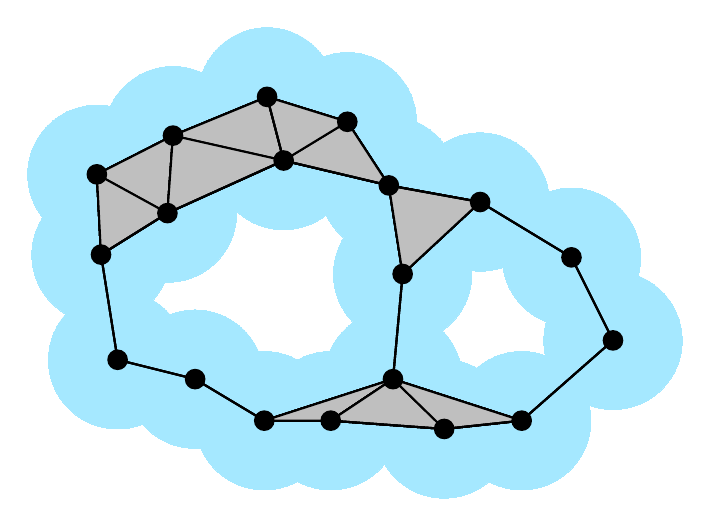
\begin{tikzpicture}[x=1pt,y=1pt,yscale=-1,xscale=1]

    \def\points{
        (111*.5,164*.5),
        (166*.5,136*.5),
        (126*.5,298*.5),
        (182*.5,312*.5),
        (114*.5,222*.5),
        (232*.5,342*.5),
        (332*.5,236*.5),
        (325*.5,312*.5),
        (280*.5,342*.5),
        (484*.5,284*.5),
        (418*.5,342*.5),
        (388*.5,184*.5),
        (292*.5,126*.5),
        (322*.5,172*.5),
        (234*.5,108*.5),
        (246*.5,154*.5),
        (162*.5,192*.5),
        (454*.5,224*.5),
        (362*.5,348*.5)
    }

    \def\r{25}

    \foreach \p in \points{
        \draw
            [color={rgb, 255:red, 165; green, 232; blue, 255}]
            [fill= {rgb, 255:red, 165; green, 232; blue, 255}]
            % [color={rgb, 255:red, 230; green, 230; blue, 230}]
            % [fill= {rgb, 255:red, 230; green, 230; blue, 230}]
            [line width=0]
            \p circle
            [radius=\r];
    }

    % \draw (100, 100) node {\(r = \r\)};

    \foreach \a [count=\ai] in \points{
        \foreach \b [count=\bi] in \points{
            \path \a;
            \pgfgetlastxy{\ax}{\ay}
            \path \b;
            \pgfgetlastxy{\bx}{\by}
            \pgfmathsetmacro\thresh{2*\r}
            \pgfmathsetmacro\distab{veclen(\ax-\bx,\ay-\by)}
            \ifnum\ai<\bi
                \ifdim\distab pt<\thresh pt
                    \draw \a -- \b;
                    \foreach \c [count=\ci] in \points{
                        \path \c;
                        \pgfgetlastxy{\cx}{\cy}
                        \pgfmathsetmacro\distac{veclen(\ax-\cx,\ay-\cy)}
                        \pgfmathsetmacro\distbc{veclen(\cx-\bx,\cy-\by)}
                        \ifdim\distac pt<\thresh pt
                            \ifdim\distbc pt<\thresh pt
                                % \draw [pattern=_iy1rqtf17,pattern size=6pt,pattern thickness=0.75pt,pattern radius=0pt, pattern color={rgb, 255:red, 50; green, 50; blue, 50}] \a -- \b -- \c -- cycle ;
                                \draw [fill=lightgray] \a -- \b -- \c -- cycle ;
                            \fi
                        \fi
                    }
                \fi
            \fi
        }
    }

    % Vertices go at the bottom so they're on top of the rest
    \foreach \p [count=\pi] in \points{
        \draw
            [black, fill=black]
            \p circle
            [radius= 3.35];
        % \draw % mark nodes for debugging
        %     [opacity=1]
        %     \p+(10,10) node {\(\p\)};
    }

\end{tikzpicture}
